
	We define another classification problem and we deal with it using SVM.
	The regularization term that we can optimize this time is the $C$ parameter, taking into account that if we use low $C$ values then the solution will be smooth, whereas if we use big $C$ values we are only interested in minimizing the error and will have a more complicated solution .
	To optimize the term on $C$ we loop on it for various values to find the most sparse $ \ alpha $ vector, ie with the greatest number of zeros, and the corresponding w model. At this point with the optimal value of $C$ and the respective model we plot the solution.
	
	\begin{figure}[h]
		\centering
		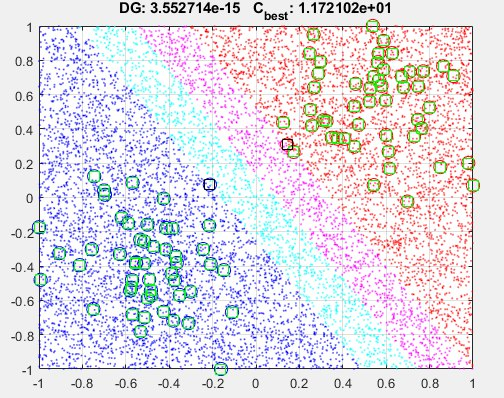
\includegraphics[width=0.5\textwidth]{i2.png}
		\caption{Regression Function}
		\label{fig:regression function}
	\end{figure}
